\chapter{系统概述}

NimlothOS是一个基于RISC-V架构实现的微型操作系统,采用Rust语言开发。系统实现了多进程支持、虚拟内存管理、文件系统、信号处理等功能。

\section{目标与特性}

NimlothOS希望在简洁的基础上实现现代操作系统的核心功能。系统具备以下主要特性:

\textbf{内存安全性:}通过Rust语言的所有权系统和类型系统,从编译期就消除了大量的内存安全问题,如缓冲区溢出、野指针访问、内存泄漏等,保障系统的稳定性和安全性。

\textbf{调度算法:}NimlothOS先实现了传统的时间片轮转调度,后来升级为多级反馈队列(MLFQ)调度算法,能够自适应地处理不同类型的工作负载,为CPU密集型和I/O密集型进程提供差异化的调度策略。

\textbf{文件系统:}支持为用户程序提供标准的文件操作接口。系统实现了自定义的Micro-FS文件系统,支持文件创建、读写、删除等基本操作,以及目录管理和路径查找功能。文件系统还提供了管道机制和标准I/O重定向,支持进程间通信和灵活的数据流处理。

\textbf{信号处理机制:}系统提供了异步事件处理能力。借鉴Unix系统的设计,NimlothOS实现了部分信号语义,支持信号的发送、接收、屏蔽和自定义处理,为异常处理和进程间通信提供了重要支撑。

\section{系统架构}

NimlothOS采用分层架构设计,从底层硬件到上层应用形成了清晰的抽象层次。每一层都有明确的职责边界,上层通过标准接口访问下层服务,实现了良好的模块化和可维护性。

\begin{figure}[htbp]
    \centering
    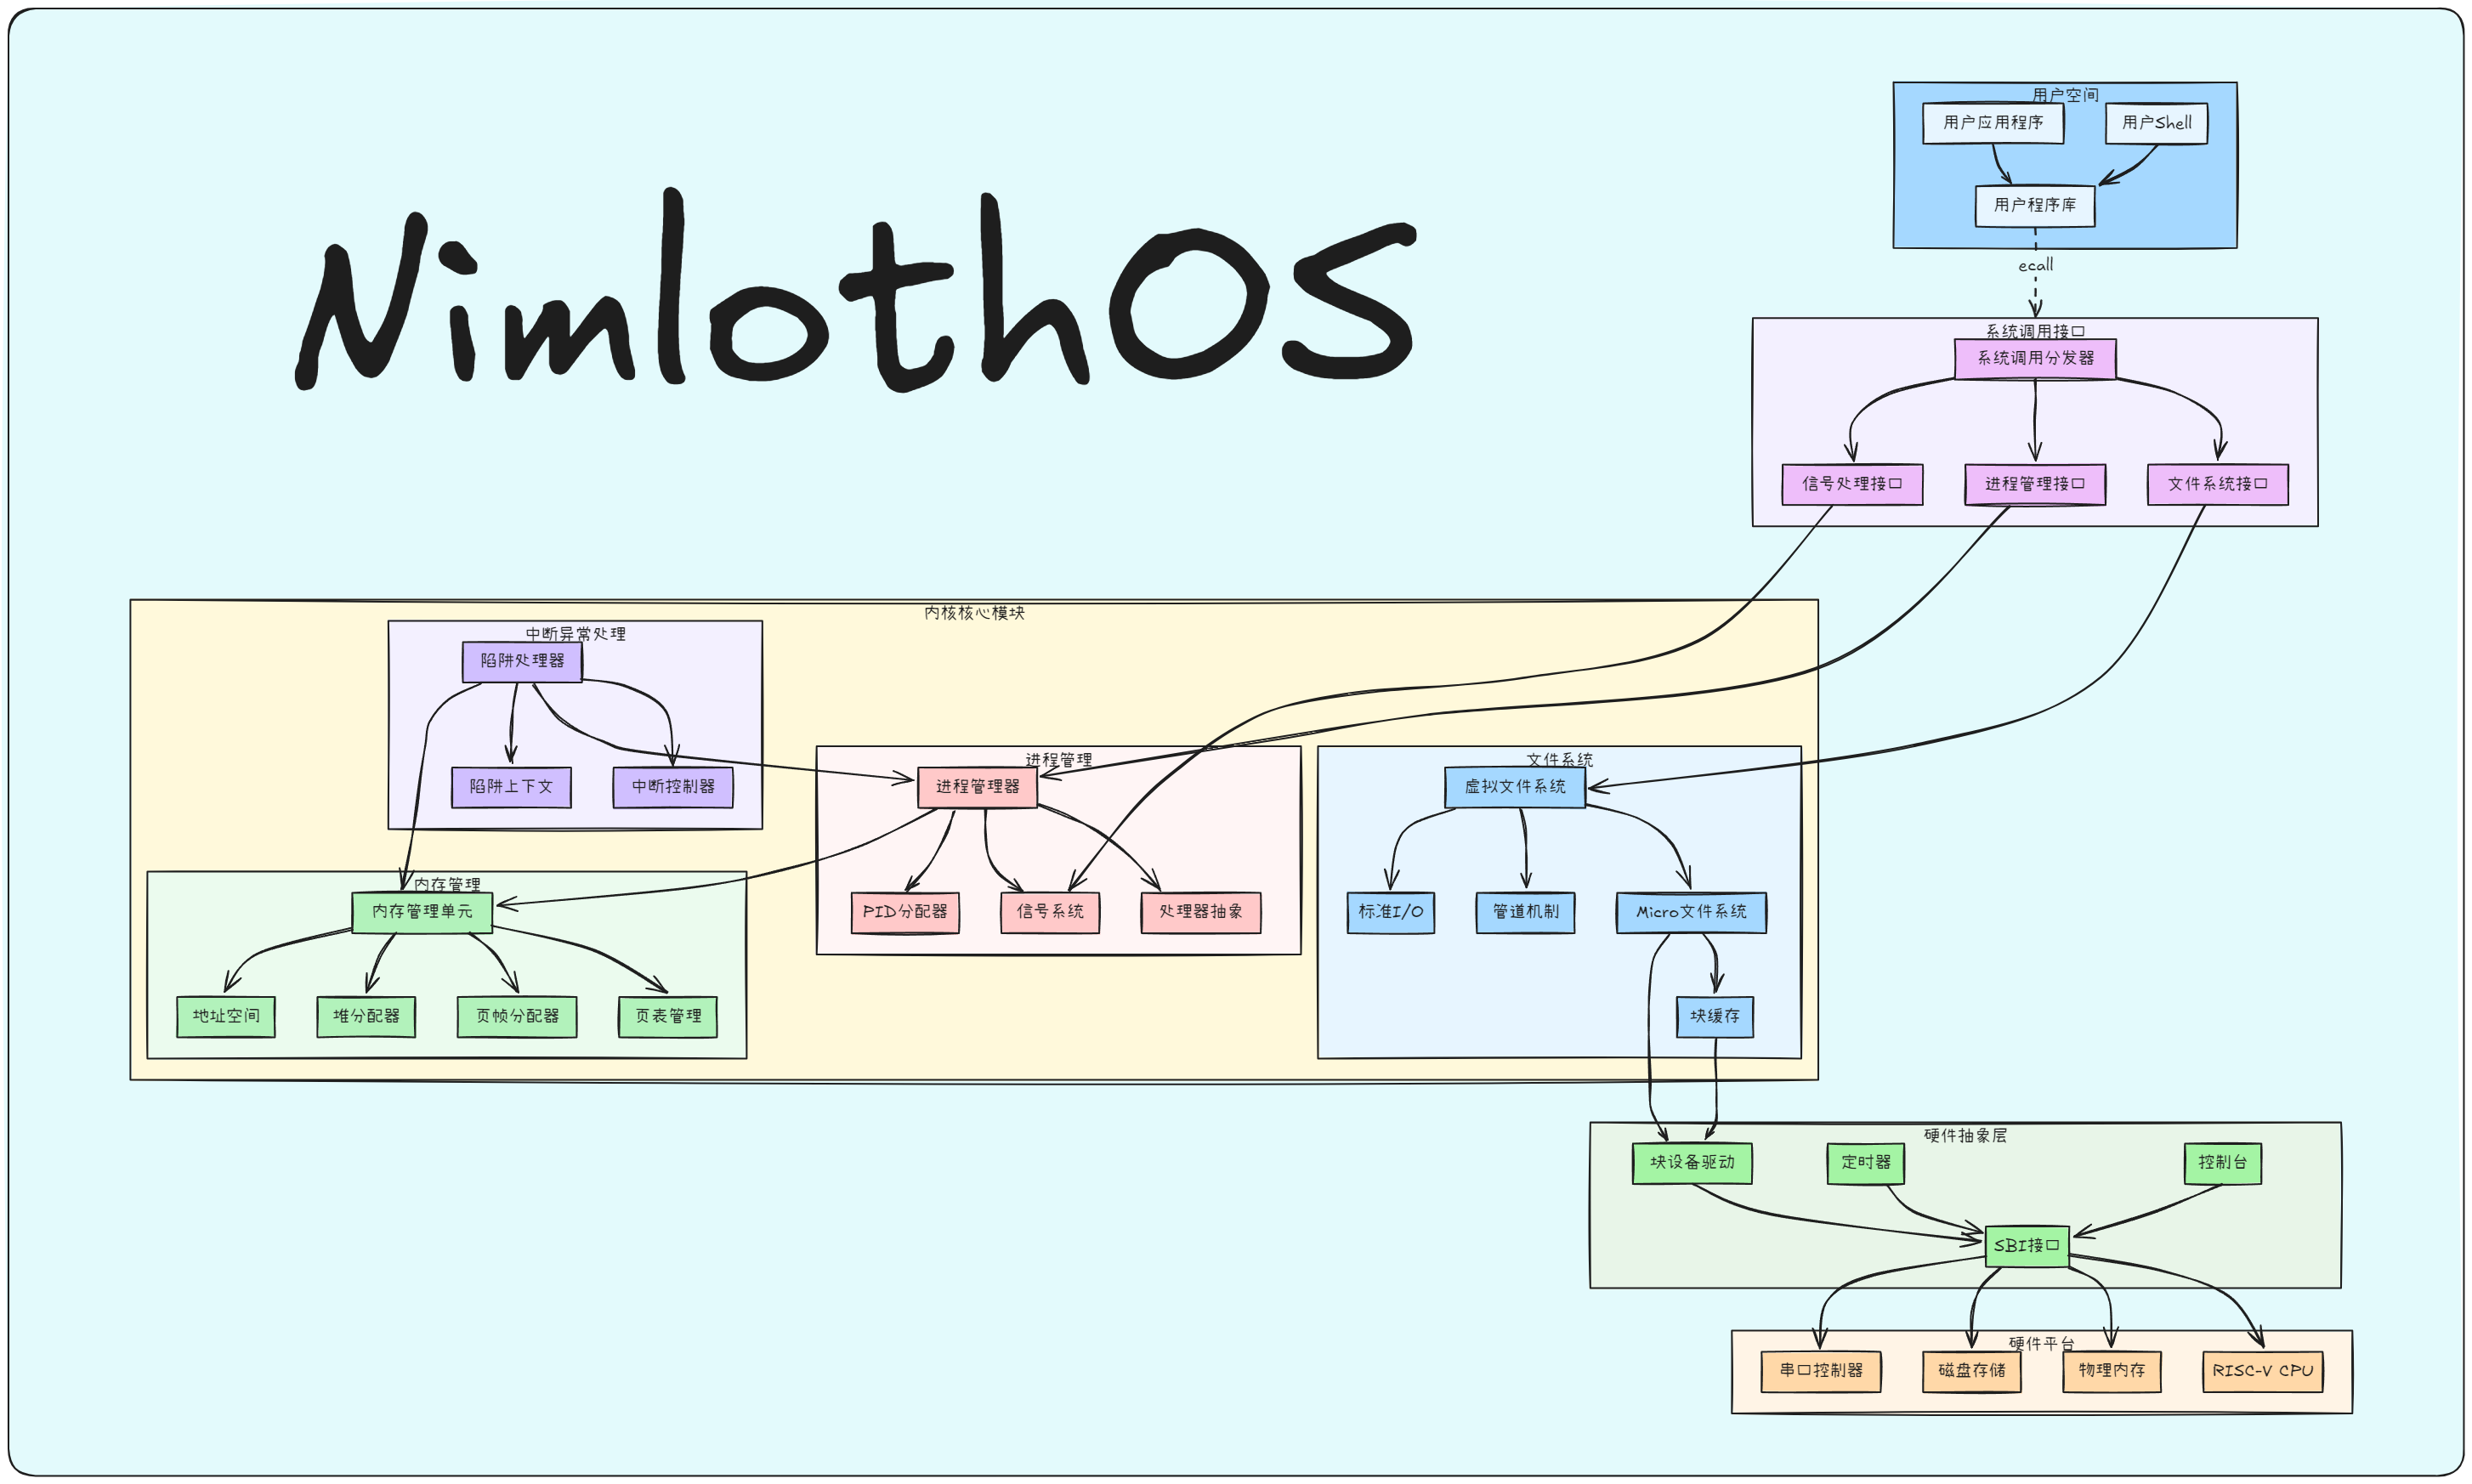
\includegraphics[width=1.0\textwidth]{../image/NimlothOS.png}
    \caption{系统架构图}
    \label{fig:architecture}
\end{figure}

\subsection{用户应用程序层}

用户应用程序层运行在用户态,包含各种用户程序和测试程序。这些程序通过系统调用接口与内核交互,获取系统服务。

\subsection{系统调用接口层}

系统调用接口层是用户态和内核态之间的桥梁,提供了POSIX风格API。接口层负责参数验证、权限检查、地址空间转换等安全性保障,确保用户程序只能通过合法途径访问系统资源。系统调用按功能分为文件系统接口、进程管理接口和信号处理接口三大类,每类都有完整的功能覆盖。

\subsection{内核核心层}

内核核心层是整个系统的核心,包含四个主要子系统:

\textbf{进程管理子系统}负责进程的创建、调度、切换和销毁。实现了基于MLFQ的调度算法,支持进程优先级动态调整,能够自适应不同类型的工作负载。子系统还包括PID管理、内核栈分配、进程间关系维护等功能。

\textbf{内存管理子系统}实现了完整的虚拟内存系统,基于RISC-V的SV39分页机制。包括三级页表管理、物理页帧分配、地址空间隔离、内核堆管理等核心功能,为进程提供了独立、安全的虚拟地址空间。

\textbf{文件系统子系统}提供了统一的文件抽象,实现了自定义的Micro-FS文件系统。支持文件和目录的基本操作、块缓存机制、管道通信、标准I/O等功能,为用户程序提供了完整的文件服务。

\textbf{中断异常处理子系统}负责处理所有的陷阱事件,包括系统调用、时钟中断、异常处理等。实现了完整的上下文保存和恢复机制,确保系统能够正确处理各种异步事件。

\subsection{硬件抽象层}

硬件抽象层通过SBI(Supervisor Binary Interface)接口为内核提供标准化的硬件访问服务。这一层屏蔽了具体硬件平台的差异,使得内核代码具有良好的可移植性。SBI提供了定时器、控制台、内存管理、电源控制等基础服务。

\subsection{硬件平台层}

硬件平台层是整个系统的物理基础,NimlothOS运行在RISC-V架构的处理器上。RISC-V是一个开放的指令集架构,具有设计简洁、模块化好、扩展性强等特点,非常适合教学和研究使用。

\section{技术特点}

NimlothOS充分利用了Rust语言的内存安全特性,在系统设计中大量运用了所有权系统、生命周期管理和类型安全机制。这些特性从根本上消除了传统C语言操作系统中常见的内存安全问题。

系统中的资源管理大量使用RAII(Resource Acquisition Is Initialization)模式,确保资源在超出作用域时自动释放。例如,物理页帧通过\texttt{FrameTracker}进行管理,进程ID通过\texttt{PidHandle}进行管理,这些设计保证了系统资源不会泄漏。

智能指针的广泛使用为系统提供了安全的内存共享机制。\texttt{Arc}和\texttt{Rc}智能指针支持引用计数的共享所有权,\texttt{UPSafeCell}提供了单处理器环境下的内部可变性,这些工具使得复杂的系统状态管理变得安全可靠。
